\documentclass[12pt,a4paper,fleqn]{article}
\usepackage[utf8]{inputenc}
\usepackage{amssymb, amsmath, multicol}
\usepackage[russian]{babel}
\usepackage{graphicx}
\usepackage[shortcuts,cyremdash]{extdash}
\usepackage{wrapfig}
\usepackage{floatflt}
\usepackage{lipsum}
\usepackage{concmath}
\usepackage{euler}
\usepackage{tikz}  
\usetikzlibrary{graphs}

\oddsidemargin=-15.4mm
\textwidth=190mm
\headheight=-32.4mm     
\textheight=277mm
\tolerance=100
\parindent=0pt
\parskip=8pt
\pagestyle{empty}
\renewcommand{\tg}{\mathop{\mathrm{tg}}\nolimits}
\renewcommand{\ctg}{\mathop{\mathrm{ctg}}\nolimits}
\renewcommand{\arctan}{\mathop{\mathrm{arctg}}\nolimits}
\newcommand{\divisible}{\mathop{\raisebox{-2pt}{\vdots}}}

\graphicspath{{pictures/}}

\begin{document}
\begin{center}
Законы Кеплера:
\end{center}
\begin{itemize}
\item 1-й закон Кеплера: \newline
Каждая планета Солнечной системы обращается по эллипсу, в одном из фокусов которого находится Солнце. Форма эллипса и степень его сходства с окружностью характеризуется отношением $e=\dfrac{c}{a}$, где $c$ — расстояние от центра эллипса до его фокуса (фокальное расстояние), $a$ — большая полуось. Величина $e$ называется эксцентриситетом эллипса. При $c = 0$, и, следовательно, $e = 0$ эллипс превращается в окружность.
\item 2-й закон Кеплера: \newline
Каждая планета движется в плоскости, проходящей через центр Солнца, причём за равные промежутки времени радиус-вектор, соединяющий Солнце и планету, описывает собой равные площади.
\item 3-й закон Кеплера: \newline
Квадраты периодов обращения планет вокруг Солнца относятся, как кубы больших полуосей орбит планет. \newline
$\dfrac{T_1^2}{T_2^2} = \dfrac{a_1^3}{a_2^3}$, \newline
где $T_1, T_2$ — периоды обращения двух планет вокруг Солнца, а $a_1, a_2$ — длины больших полуосей их орбит. Утверждение справедливо также для спутников.
\end{itemize}
Получим закон всемирного тяготения, используя законы Кеплера: \newline
1) Введем полярную систему координат с полюсом в фокусе F1, где находится Солнце и полярной осью PA, направленной вдоль большой оси эллипса (рис. 1).
\begin{center}
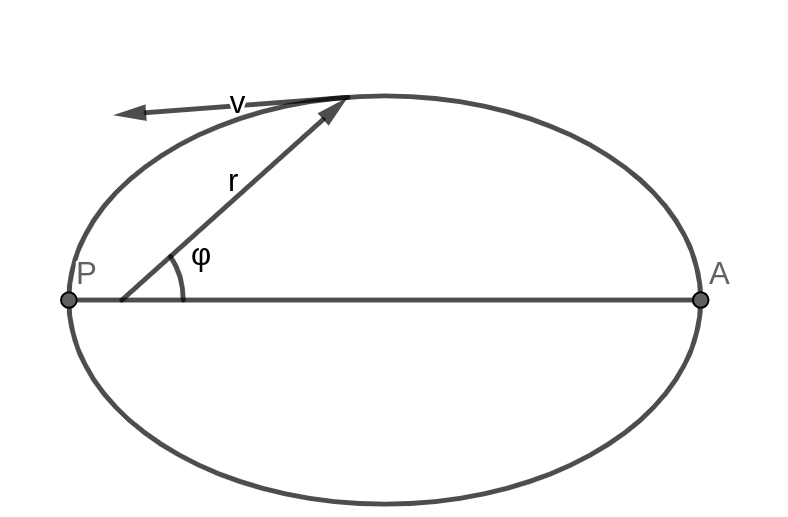
\includegraphics[scale=0.8]{geogebra-export .png}
Рис. 1
\end{center}
Ускорение движущегося тела разложим на радиальную составляющую $a_r$, направленную вдоль радиуса $r$, и азимутальную составляющую $a_{\phi}$, перпендикулярную к радиусу $r$. Они определяются выражениями:
\begin{center}
$a_r = \ddot{r} - \dot{\phi}^2r, a_{\phi} = \dfrac{1}{r}\dfrac{d}{dt} \left(r^2\dot{\phi} \right)$
\begin{flushright}
(1)
\end{flushright}
\end{center}
Докажем, что их можно записать в таком виде. Введем единичные векторы $\vec{i}, \vec{j}, \vec{k}$. Вектор $\vec{i}$ направим вдоль радиуса $r$. Вектор $\vec{j}$ перпендикулярен $\vec{i}$ и направлен в сторону возрастания угла $\phi$. Вектор $\vec{k} = [\vec{i} \vec{j}]$ (рис. 2).
\begin{center}
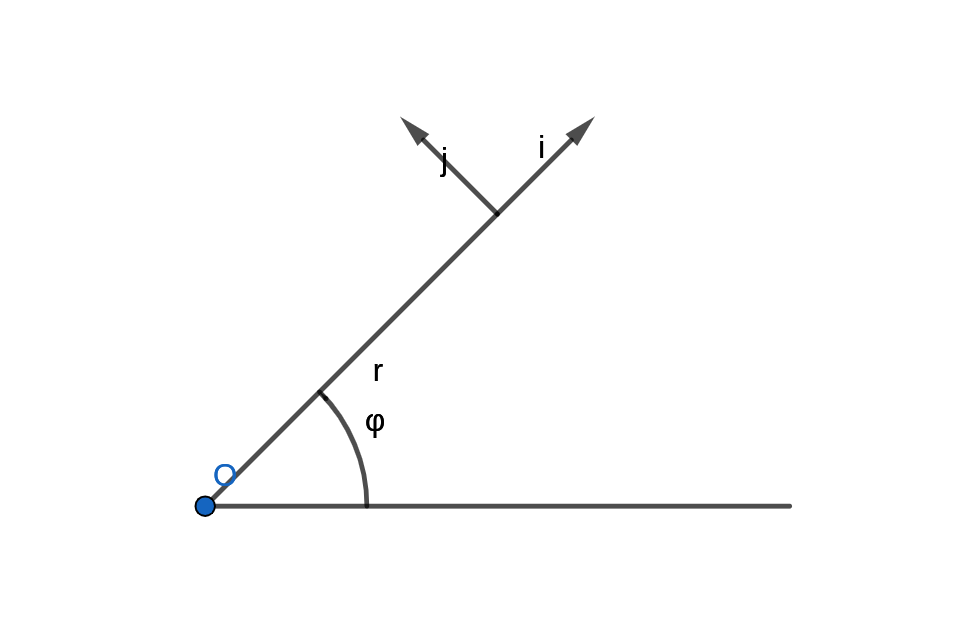
\includegraphics[scale=0.8]{geogebra-export (1).png}
Рис. 2
\end{center}
Вектор угловой скорости направлен вдоль $k$, поэтому $\omega = \dot{\phi}k$. 
\begin{center}
$\dfrac{d \vec{i}}{dt} = [\omega \vec{i}] = \dot{\phi}[\vec{k} \vec{i}] = \dot{\phi}j$, $\dfrac{d \vec{j}}{dt} = \dot{\phi}[\vec{k} \vec{j}] = -\dot{\phi} \vec{i}$ \newline
$\vec{r} = r \vec{i}$.
\begin{flushright}
(2)
\end{flushright}
\end{center}
Дифференцируем:
\begin{center}
$\vec{v} = \dot{\vec{r}} = \dot{r} \vec{i} + r \dfrac{d \vec{i}}{dt} = \dot{r} \vec{i} + r \dot{\phi} \vec{j}$
\begin{flushright}
(3)
\end{flushright}
\end{center}
Дифференцируем вторично, находим ускорение:
\begin{center}
$\vec{a} = \dot{\vec{v}} = \ddot{r} \vec{i} + r \dfrac{d \vec{i}}{dt} + \dot{r} \dot{\phi} \vec{j} + r \ddot{\phi} \vec{j} + r \dot{\phi} \dfrac{d \vec{j}}{dt} = (\ddot{r} - \dot{\phi}^2r) \vec{i} + (2 \dot{r} \dot{\phi} + r \ddot{\phi}) \vec{j} = (\ddot{r} - \dot{\phi}^2r) \vec{i} + \dfrac{1}{r}\dfrac{d}{dt} \left( r^2 \dot{\phi} \right) \vec{j}$, ч.~т.~д
\begin{flushright}
(4)
\end{flushright}
\end{center}
Величина $\sigma =  \dfrac{1}{2}r^2 \dot{\phi}$~---~секториальная скорость. По второму закону кеплера она постоянна $\rightarrow$ $a_{\phi} = 0$. Таким образом, ускорение нашего тела всегда направлено к Солнцу. 
\begin{center}
$\dot{\phi} = \dfrac{2 \sigma}{r^2}$
\begin{flushright}
(5)
\end{flushright}
\end{center} 
Вычислим $\ddot{r}$ используя уравнение конического сечения в полярной системе координат ($e$~---~эксцентриситет эллипса, $p$~---~параметр эллипса):
\begin{center}
$r(1 - e \cos \phi) = p$
\begin{flushright}
(6)
\end{flushright}
\end{center}
Продифференцируем выражение:
\begin{center}
$\dot{r}(1 - e \cos \phi) + e r \dot{\phi} \sin \phi = 0$
\begin{flushright}
(7)
\end{flushright}
\end{center}
Домножим на $r$ и воспользуемся соотношениями 5 и 6:
\begin{center}
$p \dot{r} + 2 \sigma e \sin \phi = 0$
\begin{flushright}
(8)
\end{flushright}
\end{center}
Еще раз продифференцируем:
\begin{center}
$p \ddot{r} + 2 \sigma e \cos \phi \dot{\phi} = 0$
\begin{flushright}
(9)
\end{flushright}
\end{center}
Еще раз воспользуемся соотношениями 5 и 6 и получим:
\begin{center}
$\ddot{r} = -\dfrac{4 \sigma^2}{pr^2} + \dfrac{4 \sigma^2}{r^3} = -\dfrac{4 \sigma^2}{pr^2} + \dot{\phi}^2r$
\begin{flushright}
(10)
\end{flushright}
\end{center}
Подставляем это в формулу для $a_r$:
\begin{center}
$a_r = -\dfrac{4 \sigma^2}{pr^2}$
\begin{flushright}
(11)
\end{flushright}
\end{center}
Таким образом, из законов Кеплера вытекает, что ускорение планеты обратно пропорционально квадрату ее расстояния до Солнца. \newline
2) Докажем, что коэффициент пропорциональности $\dfrac{4 \sigma^2}{p}$~---~один и тот же для всех планет. \newline
Площадь эллипса $\pi ab$, где $a, b$~---~длины большой и малой полуосей. Т.~к. секториальная скорость постоянна, то ее можно посчитать по формуле $\sigma = \dfrac{\pi ab}{T}$, где  $T$~---~период обращения планеты по ее орбите. Также воспользуемся формулой из ан. геометрии $p = \dfrac{b^2}{a}$. Тогда:
\begin{center}
$a_r = \dfrac{4 \pi^2 a^3}{T^2 r^2} = \dfrac{4 \pi^2 \mathit{K}}{r^2}$
\begin{flushright}
(12)
\end{flushright}
\end{center}
Тогда, сила, действующая на планету: 
\begin{center}
$F = \dfrac{4 \pi^2 \mathit{K} m}{r^2}$,
\begin{flushright}
(13)
\end{flushright}
\end{center} 
причем, т.~к. при описании движения Солнце и планета абсолютно равноправны, можно записать $4 \pi^2 \mathit{K} = GM$, где $M$~---~масса Солнца, $G$~---~некоторая константа. $\rightarrow$ $F = \dfrac{GMm}{r^2}$, ч.~т.~д.
\begin{center}
Задача двух тел:
\end{center}
Даны два тела (1 и 2), их начальные положения $\vec{r_1}(0), \vec{r_2}(0)$ и начальные скорости $\dot{\vec{r_1}}(0), \dot{\vec{r_2}}(0)$. Необходимо высчитать траектории $\vec{r_1}(t), \vec{r_2}(t)$. Тела взаимодействуют только друг с другом гравитационно. \newline
Обозначим $\vec{r_m} = \dfrac{\vec{r_1}m_1 + \vec{r_2}m_2}{m_1 + m_2}$~---~радиус-вектор центра масс, $\vec{r} = \vec{r_2} - \vec{r_1}$. Тогда, можно получить зависимость для $\vec{r_1}, \vec{r_2}$ через $\vec{r_m}, \vec{r}$: 
\begin{center}
$\vec{r_1} = \vec{r_m} - \dfrac{m_2}{m_1 + m_2} \vec{r}, \vec{r_2} = \vec{r_m} + \dfrac{m_1}{m_1 + m_2} \vec{r}$
\begin{flushright}
(1)
\end{flushright}
\end{center}
Вычислим $\vec{r_m}$:
\begin{center}
$\ddot{\vec{r_m}} = \dfrac{\ddot{\vec{r_1}}m_1 + \ddot{\vec{r_2}}m_2}{m_1 + m_2}$, $\ddot{\vec{r_1}}m_1 = F_{12}$, $\ddot{\vec{r_2}}m_2 = F_{21} = -F_{12} \rightarrow$ \newline
$\ddot{\vec{r_m}} = 0 \rightarrow$ \newline
$\dot{\vec{r_m}} = const = \dot{\vec{r_m}}(0) = \dfrac{\dot{\vec{r_1}}m_1 + \dot{\vec{r_2}}m_2}{m_1 + m_2} \rightarrow$ \newline
$\vec{r_m} = \vec{r_m}(0) + t \cdot \dot{\vec{r_m}}, \vec{r_m}(0) = \dfrac{\vec{r_1}m_1 + \vec{r_2}m_2}{m_1 + m_2}$
\begin{flushright}
(2)
\end{flushright}
\end{center} 
Вычислим $\vec{r}$:
\begin{center}
$\vec{r} = \vec{r_2} - \vec{r_1} \rightarrow \ddot{\vec{r}} = \ddot{\vec{r_2}} - \ddot{\vec{r_1}}$ \newline
$m_1 \ddot{\vec{r_1}} = \dfrac{\gamma m_1 m_2}{r^3} \vec{r}, m_2 \ddot{\vec{r_2}} = - \dfrac{\gamma m_1 m_2}{r^3} \vec{r} \rightarrow \ddot{\vec{r}} = -\dfrac{\gamma (m_1 + m_2)}{r^3} \vec{r}$
\begin{flushright}
(3)
\end{flushright}
\end{center}
Решением этого уравнения могут быть различные конические сечения (парабола, гипербола, эллипс). Их тип будет зависеть от накопленной энергии в системе.
\end{document}
